% Options for packages loaded elsewhere
\PassOptionsToPackage{unicode}{hyperref}
\PassOptionsToPackage{hyphens}{url}
\PassOptionsToPackage{dvipsnames,svgnames,x11names}{xcolor}
%
\documentclass[
  11pt,
]{article}
\usepackage{amsmath,amssymb}
\usepackage{lmodern}
\usepackage{iftex}
\ifPDFTeX
  \usepackage[T1]{fontenc}
  \usepackage[utf8]{inputenc}
  \usepackage{textcomp} % provide euro and other symbols
\else % if luatex or xetex
  \usepackage{unicode-math}
  \defaultfontfeatures{Scale=MatchLowercase}
  \defaultfontfeatures[\rmfamily]{Ligatures=TeX,Scale=1}
  \setmainfont[]{Palatino}
\fi
% Use upquote if available, for straight quotes in verbatim environments
\IfFileExists{upquote.sty}{\usepackage{upquote}}{}
\IfFileExists{microtype.sty}{% use microtype if available
  \usepackage[]{microtype}
  \UseMicrotypeSet[protrusion]{basicmath} % disable protrusion for tt fonts
}{}
\makeatletter
\@ifundefined{KOMAClassName}{% if non-KOMA class
  \IfFileExists{parskip.sty}{%
    \usepackage{parskip}
  }{% else
    \setlength{\parindent}{0pt}
    \setlength{\parskip}{6pt plus 2pt minus 1pt}}
}{% if KOMA class
  \KOMAoptions{parskip=half}}
\makeatother
\usepackage{xcolor}
\IfFileExists{xurl.sty}{\usepackage{xurl}}{} % add URL line breaks if available
\IfFileExists{bookmark.sty}{\usepackage{bookmark}}{\usepackage{hyperref}}
\hypersetup{
  colorlinks=true,
  linkcolor={teal},
  filecolor={Maroon},
  citecolor={teal},
  urlcolor={teal},
  pdfcreator={LaTeX via pandoc}}
\urlstyle{same} % disable monospaced font for URLs
\usepackage[left=3cm,right=3cm,top=2cm,bottom=2cm]{geometry}
\usepackage{longtable,booktabs,array}
\usepackage{calc} % for calculating minipage widths
% Correct order of tables after \paragraph or \subparagraph
\usepackage{etoolbox}
\makeatletter
\patchcmd\longtable{\par}{\if@noskipsec\mbox{}\fi\par}{}{}
\makeatother
% Allow footnotes in longtable head/foot
\IfFileExists{footnotehyper.sty}{\usepackage{footnotehyper}}{\usepackage{footnote}}
\makesavenoteenv{longtable}
\usepackage{graphicx}
\makeatletter
\def\maxwidth{\ifdim\Gin@nat@width>\linewidth\linewidth\else\Gin@nat@width\fi}
\def\maxheight{\ifdim\Gin@nat@height>\textheight\textheight\else\Gin@nat@height\fi}
\makeatother
% Scale images if necessary, so that they will not overflow the page
% margins by default, and it is still possible to overwrite the defaults
% using explicit options in \includegraphics[width, height, ...]{}
\setkeys{Gin}{width=\maxwidth,height=\maxheight,keepaspectratio}
% Set default figure placement to htbp
\makeatletter
\def\fps@figure{htbp}
\makeatother
\setlength{\emergencystretch}{3em} % prevent overfull lines
\providecommand{\tightlist}{%
  \setlength{\itemsep}{0pt}\setlength{\parskip}{0pt}}
\setcounter{secnumdepth}{-\maxdimen} % remove section numbering
\newlength{\cslhangindent}
\setlength{\cslhangindent}{1.5em}
\newlength{\csllabelwidth}
\setlength{\csllabelwidth}{3em}
\newlength{\cslentryspacingunit} % times entry-spacing
\setlength{\cslentryspacingunit}{\parskip}
\newenvironment{CSLReferences}[2] % #1 hanging-ident, #2 entry spacing
 {% don't indent paragraphs
  \setlength{\parindent}{0pt}
  % turn on hanging indent if param 1 is 1
  \ifodd #1
  \let\oldpar\par
  \def\par{\hangindent=\cslhangindent\oldpar}
  \fi
  % set entry spacing
  \setlength{\parskip}{#2\cslentryspacingunit}
 }%
 {}
\usepackage{calc}
\newcommand{\CSLBlock}[1]{#1\hfill\break}
\newcommand{\CSLLeftMargin}[1]{\parbox[t]{\csllabelwidth}{#1}}
\newcommand{\CSLRightInline}[1]{\parbox[t]{\linewidth - \csllabelwidth}{#1}\break}
\newcommand{\CSLIndent}[1]{\hspace{\cslhangindent}#1}
\usepackage[labelsep=period]{caption}
\usepackage[labelfont=bf]{caption}
\usepackage[switch]{lineno}
\usepackage{type1cm} % scalable fonts
\usepackage{lettrine}
\usepackage{booktabs}
\usepackage{sectsty} \sectionfont{\centering}
\usepackage{caption}
\captionsetup[figure]{font=footnotesize}
\captionsetup[table]{font=footnotesize}
\captionsetup[table]{justification=centerlast}
\captionsetup[figure]{justification=centerlast}
\usepackage{booktabs}
\usepackage{longtable}
\usepackage{array}
\usepackage{multirow}
\usepackage{wrapfig}
\usepackage{float}
\usepackage{colortbl}
\usepackage{pdflscape}
\usepackage{tabu}
\usepackage{threeparttable}
\usepackage{threeparttablex}
\usepackage[normalem]{ulem}
\usepackage{makecell}
\usepackage{xcolor}
\ifLuaTeX
  \usepackage{selnolig}  % disable illegal ligatures
\fi

\author{}
\date{\vspace{-2.5em}}

\begin{document}

\captionsetup{justification=raggedright,singlelinecheck=false}
\pagenumbering{gobble}

%\begin{titlepage}
\begin{center}
\begin{figure}[h!]
\centering
  
\includegraphics[width=10cm]{../images/uoy_logo.png}
  \label{}
\end{figure}
\vspace*{2\baselineskip}
\Large{\textbf{Working Title}}\\
Natasha Hopkins\\
\vspace*{2\baselineskip}
\Large{\textbf{82H Project for Master of Biology (MBiol)}}\\
\Large{Univeristy of York, UK}\\
\vspace*{2\baselineskip}
\Large{\textbf{Project Director}}\\
Dr. Richard Maguire\\
\vspace*{2\baselineskip}
\Large{\textbf{Examination Date}}\\
18 April, 2022
\end{center}

% \end{titlepage}
\hypersetup{linkcolor = black}
\newpage
\tableofcontents
\hypersetup{linkcolor = teal}

\newpage
\linenumbers
\pagenumbering{arabic}
\rule{\textwidth}{0.4pt}\\
\lettrine[lines=2,slope=0pt,nindent=0pt, loversize=0.2]{S}{hear} stress alters endothelial responses via developmental pathways. This is thought to play a role in atherosclerosis formation in regions of low shear stress. One feature of atherosclerosis is an increase in angiogenesis. \\

\begin{center}
\textbf{\textit{Key Words:}} Atherosclerosis • Wnt/βeta-catenin Signalling Pathway • Shear Stress • Orbital Shaker • Angiopoietin-2 • Thrombospondin-1\\
\end{center}

\begin{flushright}
(250 Words)\\
\end{flushright}
\rule{\textwidth}{0.4pt}

\hypertarget{introduction}{%
\section{Introduction}\label{introduction}}

Atherosclerosis is a chronic inflammatory disease characterised by the formation of arterial plaques.
Haemodynamic shear stress has been identified as a modulator of site-specificity in atherosclerosis, which occurs preferentially in regions exposed to low, oscillatory shear stress (\protect\hyperlink{ref-stone2007}{Stone et al., 2007}).
Whereas areas of high, laminar shear stress are atheroprotective (\protect\hyperlink{ref-timmins2017}{Timmins et al., 2017}).
Shear stress is an important factor in regulating gene expression in vascular endothelial cells (\protect\hyperlink{ref-Ni2010}{Ni et al., 2010}), which is thought to contribute to the susceptibility of plaque formation in atheroprone sites.
Multiple omics studies have implicated variations in flow with the regulation of developmental signalling pathways in atherosclerosis, including the Wnt Pathway (\protect\hyperlink{ref-Souilhol2020}{Souilhol et al., 2019}; \protect\hyperlink{ref-Gelfand2011}{Gelfand et al., 2011}).

Wnt is an evolutionarily conserved pathway with a critical role in axis patterning during embryonic development.
In the absence of Wnt, axin forms a destruction complex with glycogen synthase kinase 3β (GSK-3) and adenomatous polyposis coli (APC), which phosphorylates β-catenin and targets it for degradation.
However, in the active canonical Wnt pathway, Wnt ligands interact with Frizzled and LRP receptors.
This leads to the translocation of axin, inhibiting the formation of the destruction complex, allowing β-catenin to accumulate and translocate to the nucleus, where it will activate the transcription of Wnt target genes (\protect\hyperlink{ref-gordon2006}{Gordon and Nusse, 2006}).
Of these includes axin, which acts as a negative regulator of Wnt signalling (\protect\hyperlink{ref-Jho2002}{Jho et al., 2002}; \protect\hyperlink{ref-Lustig2002}{Lustig et al., 2002}).

Shear stress-mediated Wnt orchestrates a range of endothelial responses, including angiogenesis, which is increased in regions of low shear stress compared to high shear stress (\protect\hyperlink{ref-du2018}{Du and Li, 2018}).
One target of Wnt, angiopoietin-2 (ANGPT2), is an established growth factor involved in angiogenesis.
Studies in both zebrafish and mice have shown that the increase in ANGPT2 contributes to the development of atherosclerosis (\protect\hyperlink{ref-Li2014-mx}{Li et al., 2014}; \protect\hyperlink{ref-farhat2013}{Farhat et al., 2013}).

Thrombospondin-1 (THBS1) is a glycoprotein involved in endothelial cell interactions and is a potential target of Wnt.
High levels of THBS1 has been correlated with the inhibition of tumour angiogenesis (\protect\hyperlink{ref-naumov2006}{Naumov et al., 2006}), possibly by induction of apoptosis via the TGF-β pathway (\protect\hyperlink{ref-Miao2001}{Miao et al., 2001}; \protect\hyperlink{ref-yee2004}{Yee et al., 2004}), or by inhibition of the VEGF pathway (\protect\hyperlink{ref-gupta1999}{Gupta et al., 1999}; \protect\hyperlink{ref-kaur2010}{Kaur et al., 2010}).
THBS1 deficiency has also been implicated in atherosclerosis disease mice (\protect\hyperlink{ref-Moura2008}{Moura et al., 2008}).
However, little is known of the mechanism behind this.
Jo et al. (\protect\hyperlink{ref-jo2005}{2005}) demonstrated that activation of the Wnt pathway downregulates THBS1 in colon cancer, but it is not known whether WNT regulates THBS1 in atherosclerosis.
Thus, we analysed whether Wnt mediates the expression of THBS1 in response to flow.
Since atherosclerosis occurs in regions of increased angiogenesis, we would expect \emph{THSB1} to be downregulated in low shear stress.

\begin{figure}

{\centering 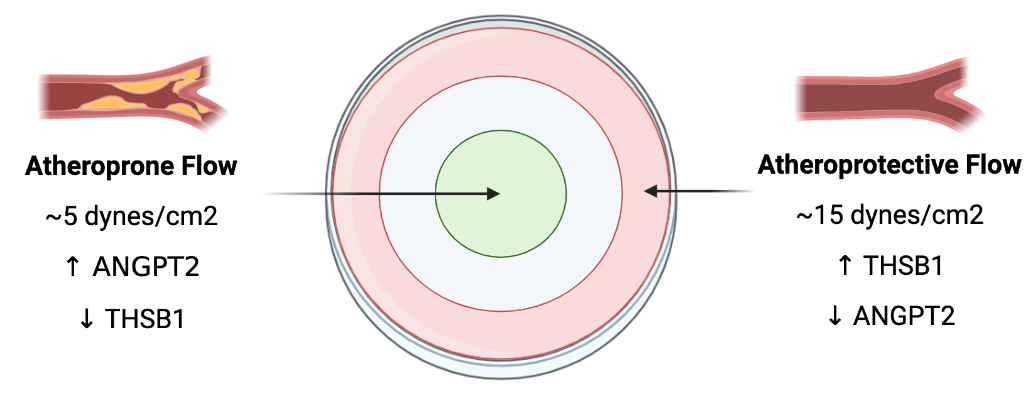
\includegraphics[width=0.8\linewidth]{../images/orbital} 

}

\caption{The orbital shaker model replicates the shear stress exterted in atheroprone and atheroprotective regions. Image created with BioRender.}\label{fig:orbital}
\end{figure}

In our study, we aimed to compare the expression of \emph{ANGPT2} and \emph{THBS1} in HUVECs exposed to atheroprone low shear stress (LSS) and atheroprotective high shear stress (HSS) using an orbital shaker model.
The model, described by Warboys et al. (\protect\hyperlink{ref-Warboys2014}{2014}), exposes cells to variable stress of approximately 5 dynes in the centre and approximately 15 dynes in the periphery of the plate (Figure \ref{fig:orbital}).
The purpose of this is to replicate the forces exerted in atheroprone and atheroprotective regions, respectively.
Based on the prior work mentioned, we expect LSS to upregulate \emph{ANGPT2} and downregulate \emph{THSB1} when compared to HSS.
We also used an inhibitor to examine whether altered expression of these genes is controlled by shear stress mediated canonical Wnt signalling.

\hypertarget{materials-and-methods}{%
\section{Materials and Methods}\label{materials-and-methods}}

\hypertarget{cell-culture-and-application-of-shear-stress}{%
\subsection{Cell Culture and Application of Shear Stress}\label{cell-culture-and-application-of-shear-stress}}

HUVECs were cultured at 37°C in 8\% M199, 0.15\% sodium bicarbonate, 1 U/mL pen-strep, 0.1 ug/ml amphotericin B, 20\% Hi-FBS, 30 ug/ml endothelial cell growth supplement (ECGS), and 10 U/ml heparin.
After reaching \textasciitilde80\% confluence, passage 2 cells were incubated with 1ml of trypsin until cells thoroughly detached, and neutralised with 9ml of M199.
They were then re-suspended in M199 media before transferring to 10mm radius 6 well plates coated in 1\% gelatin.
The canonical Wnt pathway was inhibited using XAV939.
Once confluent, cells were treated with either 3ml of 0.1\% DMSO in M199 or 0.1\% XAV939 in M199 (\protect\hyperlink{ref-Zhu2017}{Zhu et al., 2017}).
They were placed on an orbital shaker at 210 rpm for 72 hours, and exposed to low (\textasciitilde5 dynes/cm\textsuperscript{2}) and high shear stress (\textasciitilde15 dynes/cm\textsuperscript{2}) (\protect\hyperlink{ref-Warboys2019}{Warboys, Ghim and Weinberg, 2019}), with the exception of the static control.

\hypertarget{rna-extraction-and-real-time-quantitative-pcr}{%
\subsection{RNA Extraction and Real-Time Quantitative PCR}\label{rna-extraction-and-real-time-quantitative-pcr}}

Cells were isolated from the periphery and centre of the plates with cold PBS and centrifuged for 5 minutes at 400g.
Total mRNA was extracted using the RNEasy Mini Kit (Qiagen) and the concentration was determined spectrophotometrically.
cDNA synthesis was performed using the Verso cDNA Synthesis Kit (Thermo Scientific) as per the manufacturers instructions.
\emph{ANGPT2}, \emph{AXIN2}, \emph{THSB1}, and \emph{HPRT1} (reference gene) mRNA was quantified using StepOne qPCR (Thermo Scientific) with SYBR Green, using oligonucleotide qPCR primers from Ensembl (\protect\hyperlink{ref-howe2020}{Howe et al., 2020}) (Table \ref{tab:primers}).
The amplification included 30 cycles at 95°C for 30s, 5°C for 30s, and 72°C for 45s, followed by 72 °C 10 min.

\begin{table}[!h]

\caption{\label{tab:primers}Oligonucleotide qPCR primers from Ensembl.}
\begin{tabu} to \linewidth {>{\raggedright}X>{\raggedright}X>{\raggedright\arraybackslash}p{8cm}}
\toprule
Gene & Direction & Sequence\\
\midrule
 & L & CGGCTGTGATGATAGAAATAGGGA\\

\multirow{-2}{*}{\raggedright\arraybackslash ANGPT2} & R & GTTCCAAGAGCTGAAGTTCAAGTC\\

 & L & TGTCACTTACTTTTTCTGTGGGGA\\

\multirow{-2}{*}{\raggedright\arraybackslash AXIN1} & R & TGTCACTTACTTTTTCTGTGGGGA\\

 & L & TTGGTCAGGCAGTATAATCC\\

\multirow{-2}{*}{\raggedright\arraybackslash HPRT1} & R & GGGCATATCCTACAACAAC\\

 & L & AAAGATGGAGAATGCTGAGTTGGA\\

\multirow{-2}{*}{\raggedright\arraybackslash THSB1} & R & GGTTCCAAAGACAAACCTCACATT\\
\bottomrule
\end{tabu}
\end{table}

\hypertarget{statistical-analysis}{%
\subsection{Statistical Analysis}\label{statistical-analysis}}

Relative expression is expressed as 2\textsuperscript{ΔΔCt} fold change ± SEM, normalised to the HPRT control.
Normality was determined with Kolmogorov-Smirnov Tests.
Comparison analysis was performed using the Student's t-test.
All plots and analyses were performed in R (\protect\hyperlink{ref-R}{R Core Team, 2018}).

\hypertarget{results-rewrite-make-clearer}{%
\section{Results REWRITE MAKE CLEARER}\label{results-rewrite-make-clearer}}

To asses the effect of low and high shear stress on gene express, HUVECs were exposed to flow using an orbital shaker system.
Gene expression of \emph{ANGPT2}, \emph{THSB1}, and Wnt reporter \emph{AXIN2} was quantified by qPCR.
Gene expression in HUVECs exposed LSS was compared to those exposed to HSS (Figure \ref{fig:plots}A).
Low shear stress downregulated the expression of \emph{AXIN2}, \emph{ANGPT2}, and \emph{THBS1}.
\emph{AXIN2}, a known Wnt target, decreased by 0.28-fold in low shear stress.
Similarly, \emph{ANGPT2} was decreased by 0.15-fold, and THBS1 was decreased 0.12-fold.

Using the same method, HUVECs were also treated with either DMSO or canonical Wnt inhibitor XAV929, to assess for regulation by Wnt signalling.
Expression in the presence of XAV939 was then compared to DMSO (Figure \ref{fig:plots}B).
Exposure to LSS with the addition XAV939 intensified the expression of \emph{AXIN2} by 18.82-fold, \emph{ANGPT} by 33.35-fold, and \emph{THBS1} by 35.59-fold.
Whereas XAV929 decreased expression in HSS.
\emph{AXIN2} decreased 0.68-fold, \emph{ANGPT2} by 0.42-fold, and \emph{THBS1} by 0.87-fold.
Results were analysed using the Students \emph{t} test, which regarded them insignificant due to the small sample size.

\begin{figure}

{\centering 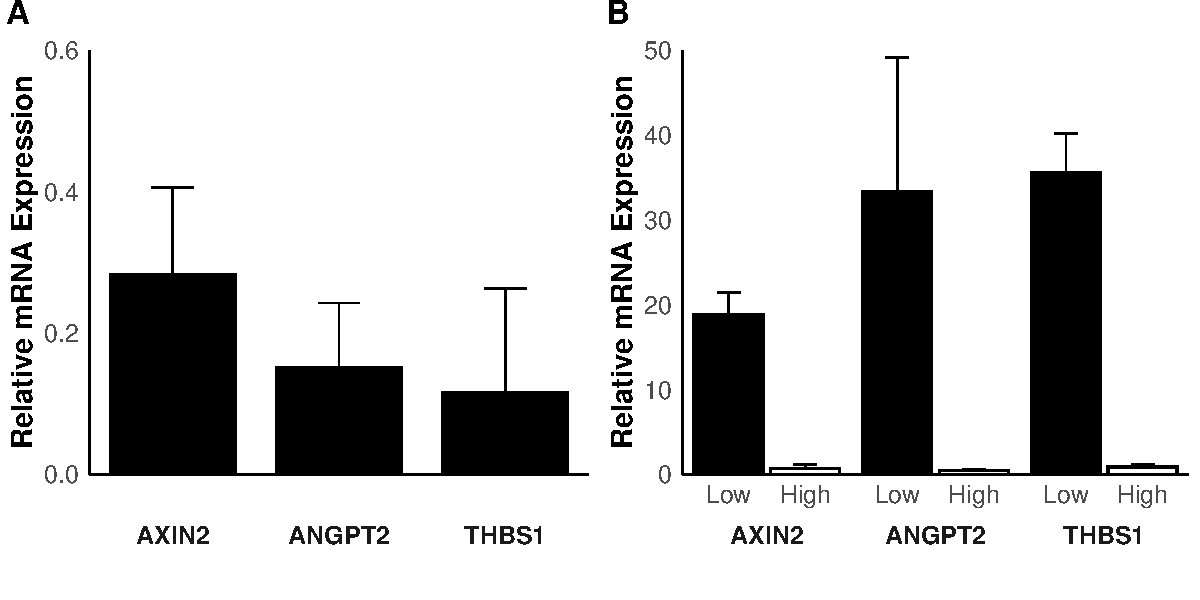
\includegraphics{report_files/figure-latex/plots-1} 

}

\caption{Low shear stress downregulates AXIN2, ANGPT2, and THSB1 expression via Wnt signalling. Cells were treated with DMSO(-) or XAV939(+) and exposed to low or high shear stress. Levels of angiopoietin-2, axin-2, and thrombospondin-1 mRNA were quantified by qPCR. (\textbf{A}) Low shear stress upregulated the expression of all genes. \emph{AXIN}: 0.28±0.12, \emph{ANGPT2}: 0.15±0.09, \emph{THBS1}: 0.12±0.15. Data is shown as fold change ± SEM of low shear stress relative to high shear stress. (\textbf{B}) XAV939 upregulated expression of all genes in low shear stress and downregulated expression of all genes in high shear stress. \emph{AXIN}: 18.82±2.66 and 0.68±0.50. \emph{ANGPT2}: 33.36±15.80 and 0.42±0.14, \emph{THBS1}: 35.59±4.55 and 0.87±0.33. Data is shown as fold change ± SEM of XAV939 relative to DMSO.}\label{fig:plots}
\end{figure}

\hypertarget{discussion}{%
\section{Discussion}\label{discussion}}

In our study, we analyse the effects of low shear stress and high shear stress on the expression of two regulators of angiogenesis, \emph{ANGPT2} and \emph{THBS1}, and whether their expression is controlled by Wnt.
This was achieved using an orbital shaker model, first described by Warboys et al. (\protect\hyperlink{ref-Warboys2014}{2014}).
Direct Wnt target, \emph{AXIN2}, was also measured to quantify Wnt expression (\protect\hyperlink{ref-Jho2002}{Jho et al., 2002}).
Finally, we compared gene expression in LSS to HSS, and XAV939 to DMSO.

Our findings indicate that \emph{AXIN2}, \emph{ANGPT}, and \emph{THBS1} is downregulated in HUVECs exposed to LSS (Figure \ref{fig:plots}A).
The downregulation of \emph{ANGPT} and \emph{AXIN2} in LSS differs from our expectations.
Previous studies demonstrate that canonical Wnt is activated by low shear stress (\protect\hyperlink{ref-Gelfand2011}{Gelfand et al., 2011}), as is its direct target, \emph{AXIN2} (\protect\hyperlink{ref-Jho2002}{Jho et al., 2002}).
\emph{ANGPT2}, a positive regulator of angiogenesis, has also been identified as a positive target of Wnt in zebrafish (\protect\hyperlink{ref-Li2014-mx}{Li et al., 2014}).
Thus, \emph{ANGPT2} was also expected to be upregulated in LSS.
However, the results imply that Wnt is downregulated by LSS compared to HSS, and in doing so, downregulates both \emph{ANGPT2} and \emph{AXIN2}.

Conversely, the lower expression of \emph{THSB1} in low shear stress was anticipated --- Moura et al. (\protect\hyperlink{ref-Moura2008}{2008}) demonstrated that \emph{THBS1} deficiency accelerated plaque formation in atherosclerosis.
In colonic tumours, \emph{THBS1} expression is mediated by Wnt signalling.
We assessed whether this was the case in atherosclerosis.
However, \emph{THBS1} increased in the presence of XAV939, suggesting that it is upregulated by the Wnt pathway.

In the presence of inhibitor XAV939, all genes were upregulated in LSS and downregulated in HSS (Figure \ref{fig:plots}B).
Initially, this would imply that canonical Wnt inhibits \emph{ANGPT2} and \emph{THSB1}.
However, since \emph{AXIN2} is a direct target of canonical Wnt, it could be that the inhibitor failed.
Inhibition of canonical Wnt signalling leads to the phosphorylation of β-catenin, targeting it for degradation.
Therefore, inhibitor efficiency can be assessed using a Western blot with antibodies targeting β-catenin and phospho-β-catenin, comparing their abundance after treatment with DMSO or XAV939 (\protect\hyperlink{ref-Huang2009}{Huang et al., 2009}).
If XAV939 is functioning, we will see a decrease in β-catenin and increase phospho-β-catenin.

On the other hand, the possibility of XAV939 failure is contradicted by the DMSO and XAV939 results; if canonical Wnt is not inhibited, we would expect the XAV939 sample to reflect cells that were treated DMSO, but this was not the case.
This could be explained by a fault in the specificity of our primers for \emph{AXIN2}, \emph{ANGPT2}, and \emph{THSB1}.
For instance, the primers may also target other flow mediated genes that are downregulated by Wnt.
Thus, falsely altering the abundance of the genes when treated with XAV939.
In addition to this, qPCR melt curves imply that there were primer dimers, therefore, more optimal primers should be used.
Primer specificity could be ensured using melt curve analysis with serial dilutions.
Alternatively, previously published primers could be used (\protect\hyperlink{ref-Li2014-mx}{Li et al., 2014}; \protect\hyperlink{ref-lopes2003}{Lopes et al., 2003}).

\begin{center}\rule{0.5\linewidth}{0.5pt}\end{center}

\hypertarget{interactions-with-other-pathways}{%
\subsection{Interactions With Other Pathways}\label{interactions-with-other-pathways}}

**What is WNT5a Pathway/calcium)

``PKC, activated by the Wnt-Ca\textsuperscript{2+} signaling pathway blocks the canonical pathway upstream of β-catenin by phosphorylating DSH (\href{https://www.sciencedirect.com/science/article/pii/S0021915014013549\#fig1}{Fig.1}).'' (\protect\hyperlink{ref-Mikels2006}{Mikels and Nusse, 2006})

Non-canonical Wnt signalling are less established pathways which do not involve β-catenin.
Wnt5a is a glycoprotein which activates the non-canonical Wnt-Ca\textsuperscript{2+} pathway, which stimulates Ca\textsuperscript{2+} release from the endoplasmic reticulum (\protect\hyperlink{ref-Kohn2005}{Kohn and Moon, 2005}). Wnt5a is upregulated in advanced atherosclerotic lesions (\protect\hyperlink{ref-Bhatt2012}{M. Bhatt, 2012}; \protect\hyperlink{ref-Christman2008}{Christman et al., 2008}) and other conditions associated with increased risk of atherosclerosis, such as obesity (\protect\hyperlink{ref-karki2017}{Karki et al., 2017}; \protect\hyperlink{ref-fuster2014}{Fuster et al., 2014}) and diabetes(\protect\hyperlink{ref-Li2021}{Li et al., 2021}; \protect\hyperlink{ref-Xu2020}{Xu et al., 2020}).

Wnt5a has also been shown to antagonize canonical Wnt by inhibiting β-catenin reporter gene expression (\protect\hyperlink{ref-Mikels2006}{Mikels and Nusse, 2006}), but the mechanism behind this is unclear.

-- MECHANISM SUGGESTIONS ---

Therefore, an increase in Wnt5a in low shear stress could decrease canonical-Wnt signalling, explaining the downregulation of all 3 genes in response to LSS.

Despite it's potential to inhibit pro-angiogenic canonical-Wnt, Wnt5a

has been shown to upregulate expression of Tie-2, an angiopoietin receptor.

Many previous studies

\begin{center}\rule{0.5\linewidth}{0.5pt}\end{center}

\hypertarget{future-directions}{%
\subsection{Future Directions}\label{future-directions}}

There are many discrepancies between our results and prior studies, likely due to limitations and errors in our method.

Firstly, our sample size was extremely small, and did not include biological replicates, so our results cannot be generalised.
For our work to be generalisable, HUVECs from multiple donors should be used, so that there are both biological and technical repeats.

One issue with our model is the lack of distinction between cells exposed to low or high shear stress; as both of these cells inhabit the same plate, there is a high risk of cross-contamination.
A solution to this would be using non-adherent PEG-gel to selectively grow cells in either the centre or periphery of the plates (\protect\hyperlink{ref-Fernandes2022}{Fernandes et al., 2022}).

Another limitation of the orbital shaker is that it exerts non-uniform stress, so the levels of shear stress can only be estimated.

Arguably most importantly, the majority previous studies are conducted in vivo with either zebrafish or mice.
So, our results may be exclusive to our in vitro orbital shaker model with HUVECs.

\begin{center}\rule{0.5\linewidth}{0.5pt}\end{center}

\hypertarget{acknowledgements}{%
\section{Acknowledgements}\label{acknowledgements}}

\begin{flushright}
Word Count: 1826 Words
\end{flushright}

\hypertarget{references}{%
\section{References}\label{references}}

\small

\hypertarget{refs}{}
\begin{CSLReferences}{0}{0}
\leavevmode\vadjust pre{\hypertarget{ref-Christman2008}{}}%
\CSLLeftMargin{1. }
\CSLRightInline{Christman, M. A. {et al.} (2008). {Wnt5a is expressed in murine and human atherosclerotic lesions}. \emph{American Journal of Physiology-Heart and Circulatory Physiology}, 294 (6), pp.H2864--H2870. {[}Online{]}. Available at: doi:\href{https://doi.org/10.1152/ajpheart.00982.2007}{10.1152/ajpheart.00982.2007}.}

\leavevmode\vadjust pre{\hypertarget{ref-du2018}{}}%
\CSLLeftMargin{2. }
\CSLRightInline{Du, J. and Li, J. (2018). {The role of wnt signaling pathway in atherosclerosis and its relationship with angiogenesis}. \emph{Experimental and Therapeutic Medicine}. {[}Online{]}. Available at: doi:\href{https://doi.org/10.3892/etm.2018.6397}{10.3892/etm.2018.6397}.}

\leavevmode\vadjust pre{\hypertarget{ref-farhat2013}{}}%
\CSLLeftMargin{3. }
\CSLRightInline{Farhat, N. {et al.} (2013). {Angiopoietin{-}Like 2 Promotes Atherogenesis in Mice}. \emph{Journal of the American Heart Association}, 2 (3). {[}Online{]}. Available at: doi:\href{https://doi.org/10.1161/jaha.113.000201}{10.1161/jaha.113.000201}.}

\leavevmode\vadjust pre{\hypertarget{ref-Fernandes2022}{}}%
\CSLLeftMargin{4. }
\CSLRightInline{Fernandes, A. {et al.} (2022). {Engineering solutions for biological studies of flow-exposed endothelial cells on orbital shakers}. Maghsoudlou, P. (Ed). \emph{PLOS ONE}, 17 (1), p.e0262044. {[}Online{]}. Available at: doi:\href{https://doi.org/10.1371/journal.pone.0262044}{10.1371/journal.pone.0262044}.}

\leavevmode\vadjust pre{\hypertarget{ref-fuster2014}{}}%
\CSLLeftMargin{5. }
\CSLRightInline{Fuster, J. J. {et al.} (2014). {Noncanonical Wnt Signaling Promotes Obesity-Induced Adipose Tissue Inflammation and Metabolic Dysfunction Independent of Adipose Tissue Expansion}. \emph{Diabetes}, 64 (4), pp.1235--1248. {[}Online{]}. Available at: doi:\href{https://doi.org/10.2337/db14-1164}{10.2337/db14-1164}.}

\leavevmode\vadjust pre{\hypertarget{ref-Gelfand2011}{}}%
\CSLLeftMargin{6. }
\CSLRightInline{Gelfand, B. D. {et al.} (2011). {Hemodynamic Activation of β-Catenin and T-Cell-Specific Transcription Factor Signaling in Vascular Endothelium Regulates Fibronectin Expression}. \emph{Arteriosclerosis, Thrombosis, and Vascular Biology}, 31 (7), pp.1625--1633. {[}Online{]}. Available at: doi:\href{https://doi.org/10.1161/atvbaha.111.227827}{10.1161/atvbaha.111.227827}.}

\leavevmode\vadjust pre{\hypertarget{ref-gordon2006}{}}%
\CSLLeftMargin{7. }
\CSLRightInline{Gordon, M. D. and Nusse, R. (2006). {Wnt Signaling: Multiple Pathways, Multiple Receptors, and Multiple Transcription Factors}. \emph{Journal of Biological Chemistry}, 281 (32), pp.22429--22433. {[}Online{]}. Available at: doi:\href{https://doi.org/10.1074/jbc.r600015200}{10.1074/jbc.r600015200}.}

\leavevmode\vadjust pre{\hypertarget{ref-gupta1999}{}}%
\CSLLeftMargin{8. }
\CSLRightInline{Gupta, K. {et al.} (1999). \emph{Angiogenesis}, 3 (2), pp.147--158. {[}Online{]}. Available at: doi:\href{https://doi.org/10.1023/a:1009018702832}{10.1023/a:1009018702832}.}

\leavevmode\vadjust pre{\hypertarget{ref-howe2020}{}}%
\CSLLeftMargin{9. }
\CSLRightInline{Howe, K. L. {et al.} (2020). {Ensembl 2021}. \emph{Nucleic Acids Research}, 49 (D1), pp.D884--D891. {[}Online{]}. Available at: doi:\href{https://doi.org/10.1093/nar/gkaa942}{10.1093/nar/gkaa942}.}

\leavevmode\vadjust pre{\hypertarget{ref-Huang2009}{}}%
\CSLLeftMargin{10. }
\CSLRightInline{Huang, S.-M. A. {et al.} (2009). {Tankyrase inhibition stabilizes axin and antagonizes Wnt signalling}. \emph{Nature}, 461 (7264), pp.614--620. {[}Online{]}. Available at: doi:\href{https://doi.org/10.1038/nature08356}{10.1038/nature08356}.}

\leavevmode\vadjust pre{\hypertarget{ref-Jho2002}{}}%
\CSLLeftMargin{11. }
\CSLRightInline{Jho, E. {et al.} (2002). {Wnt/β-Catenin/Tcf Signaling Induces the Transcription of Axin2, a Negative Regulator of the Signaling Pathway}. \emph{Molecular and Cellular Biology}, 22 (4), pp.1172--1183. {[}Online{]}. Available at: doi:\href{https://doi.org/10.1128/mcb.22.4.1172-1183.2002}{10.1128/mcb.22.4.1172-1183.2002}.}

\leavevmode\vadjust pre{\hypertarget{ref-jo2005}{}}%
\CSLLeftMargin{12. }
\CSLRightInline{Jo, W.-S. {et al.} (2005). {Wnt signaling can repress thrombospondin-1 expression in colonic tumorigenesis}. \emph{Cancer Biology \& Therapy}, 4 (12), pp.1361--1366. {[}Online{]}. Available at: doi:\href{https://doi.org/10.4161/cbt.4.12.2201}{10.4161/cbt.4.12.2201}.}

\leavevmode\vadjust pre{\hypertarget{ref-karki2017}{}}%
\CSLLeftMargin{13. }
\CSLRightInline{Karki, S. {et al.} (2017). {WNT5A regulates adipose tissue angiogenesis via antiangiogenic VEGF-A{\textsubscript{165}}b in obese humans}. \emph{American Journal of Physiology-Heart and Circulatory Physiology}, 313 (1), pp.H200--H206. {[}Online{]}. Available at: doi:\href{https://doi.org/10.1152/ajpheart.00776.2016}{10.1152/ajpheart.00776.2016}.}

\leavevmode\vadjust pre{\hypertarget{ref-kaur2010}{}}%
\CSLLeftMargin{14. }
\CSLRightInline{Kaur, S. {et al.} (2010). {Thrombospondin-1 Inhibits VEGF Receptor-2 Signaling by Disrupting Its Association with CD47}. \emph{Journal of Biological Chemistry}, 285 (50), pp.38923--38932. {[}Online{]}. Available at: doi:\href{https://doi.org/10.1074/jbc.m110.172304}{10.1074/jbc.m110.172304}.}

\leavevmode\vadjust pre{\hypertarget{ref-Kohn2005}{}}%
\CSLLeftMargin{15. }
\CSLRightInline{Kohn, A. D. and Moon, R. T. (2005). {Wnt and calcium signaling: β-Catenin-independent pathways}. \emph{Cell Calcium}, 38 (3-4), pp.439--446. {[}Online{]}. Available at: doi:\href{https://doi.org/10.1016/j.ceca.2005.06.022}{10.1016/j.ceca.2005.06.022}.}

\leavevmode\vadjust pre{\hypertarget{ref-Li2014-mx}{}}%
\CSLLeftMargin{16. }
\CSLRightInline{Li, R. {et al.} (2014). {Shear stress-activated wnt-angiopoietin-2 signaling recapitulates vascular repair in zebrafish embryos}. \emph{Arteriosclerosis, thrombosis, and vascular biology}, 34 (10), pp.2268--2275.}

\leavevmode\vadjust pre{\hypertarget{ref-Li2021}{}}%
\CSLLeftMargin{17. }
\CSLRightInline{Li, X. {et al.} (2021). {Wnt5a promotes renal tubular inflammation in diabetic nephropathy by binding to CD146 through noncanonical Wnt signaling}. \emph{Cell Death \& Disease}, 12 (1). {[}Online{]}. Available at: doi:\href{https://doi.org/10.1038/s41419-020-03377-x}{10.1038/s41419-020-03377-x}.}

\leavevmode\vadjust pre{\hypertarget{ref-lopes2003}{}}%
\CSLLeftMargin{18. }
\CSLRightInline{Lopes, N. {et al.} (2003). {Thrombospondin 2 Regulates Cell Proliferation Induced by Rac1 Redox-Dependent Signaling}. \emph{Molecular and Cellular Biology}, 23 (15), pp.5401--5408. {[}Online{]}. Available at: doi:\href{https://doi.org/10.1128/mcb.23.15.5401-5408.2003}{10.1128/mcb.23.15.5401-5408.2003}.}

\leavevmode\vadjust pre{\hypertarget{ref-Lustig2002}{}}%
\CSLLeftMargin{19. }
\CSLRightInline{Lustig, B. {et al.} (2002). {Negative Feedback Loop of Wnt Signaling through Upregulation of Conductin/Axin2 in Colorectal and Liver Tumors}. \emph{Molecular and Cellular Biology}, 22 (4), pp.1184--1193. {[}Online{]}. Available at: doi:\href{https://doi.org/10.1128/mcb.22.4.1184-1193.2002}{10.1128/mcb.22.4.1184-1193.2002}.}

\leavevmode\vadjust pre{\hypertarget{ref-Bhatt2012}{}}%
\CSLLeftMargin{20. }
\CSLRightInline{M. Bhatt, P. (2012). {Increased Wnt5a mRNA Expression in Advanced Atherosclerotic Lesions, and Oxidized LDL Treated Human Monocyte-Derived Macrophages}. \emph{The Open Circulation and Vascular Journal}, 5 (1), pp.1--7. {[}Online{]}. Available at: doi:\href{https://doi.org/10.2174/1877382601205010001}{10.2174/1877382601205010001}.}

\leavevmode\vadjust pre{\hypertarget{ref-Miao2001}{}}%
\CSLLeftMargin{21. }
\CSLRightInline{Miao, W. M. {et al.} (2001). {Thrombospondin-1 type 1 repeat recombinant proteins inhibit tumor growth through transforming growth factor-beta-dependent and -independent mechanisms.} \emph{Cancer research}, 61 21, pp.7830--7839.}

\leavevmode\vadjust pre{\hypertarget{ref-Mikels2006}{}}%
\CSLLeftMargin{22. }
\CSLRightInline{Mikels, A. J. and Nusse, R. (2006). {Purified Wnt5a Protein Activates or Inhibits β-Catenin{\textendash}TCF Signaling Depending on Receptor Context}. Arias, A. M. (Ed). \emph{PLoS Biology}, 4 (4), p.e115. {[}Online{]}. Available at: doi:\href{https://doi.org/10.1371/journal.pbio.0040115}{10.1371/journal.pbio.0040115}.}

\leavevmode\vadjust pre{\hypertarget{ref-Moura2008}{}}%
\CSLLeftMargin{23. }
\CSLRightInline{Moura, R. {et al.} (2008). {Thrombospondin-1 Deficiency Accelerates Atherosclerotic Plaque Maturation in {\emph{ApoE}} {\textsuperscript{{-}/{-}}} Mice}. \emph{Circulation Research}, 103 (10), pp.1181--1189. {[}Online{]}. Available at: doi:\href{https://doi.org/10.1161/circresaha.108.185645}{10.1161/circresaha.108.185645}.}

\leavevmode\vadjust pre{\hypertarget{ref-naumov2006}{}}%
\CSLLeftMargin{24. }
\CSLRightInline{Naumov, G. N. {et al.} (2006). {A Model of Human Tumor Dormancy: An Angiogenic Switch From the Nonangiogenic Phenotype}. \emph{JNCI: Journal of the National Cancer Institute}, 98 (5), pp.316--325. {[}Online{]}. Available at: doi:\href{https://doi.org/10.1093/jnci/djj068}{10.1093/jnci/djj068}.}

\leavevmode\vadjust pre{\hypertarget{ref-Ni2010}{}}%
\CSLLeftMargin{25. }
\CSLRightInline{Ni, C.-W. {et al.} (2010). {Discovery of novel mechanosensitive genes in vivo using mouse carotid artery endothelium exposed to disturbed flow}. \emph{Blood}, 116 (15), pp.e66--e73. {[}Online{]}. Available at: doi:\href{https://doi.org/10.1182/blood-2010-04-278192}{10.1182/blood-2010-04-278192}.}

\leavevmode\vadjust pre{\hypertarget{ref-R}{}}%
\CSLLeftMargin{26. }
\CSLRightInline{R Core Team. (2018). {\emph{R: A language and environment for statistical computing}}. Vienna, Austria: R Foundation for Statistical Computing. {[}Online{]}. Available at: \url{https://www.R-project.org/}.}

\leavevmode\vadjust pre{\hypertarget{ref-Souilhol2020}{}}%
\CSLLeftMargin{27. }
\CSLRightInline{Souilhol, C. {et al.} (2019). {Endothelial responses to shear stress in atherosclerosis: a novel role for developmental genes}. \emph{Nature Reviews Cardiology}, 17 (1), pp.52--63. {[}Online{]}. Available at: doi:\href{https://doi.org/10.1038/s41569-019-0239-5}{10.1038/s41569-019-0239-5}.}

\leavevmode\vadjust pre{\hypertarget{ref-stone2007}{}}%
\CSLLeftMargin{28. }
\CSLRightInline{Stone, P. H. {et al.} (2007). {Regions of low endothelial shear stress are the sites where coronary plaque progresses and vascular remodelling occurs in humans: an in vivo serial study}. \emph{European Heart Journal}, 28 (6), pp.705--710. {[}Online{]}. Available at: doi:\href{https://doi.org/10.1093/eurheartj/ehl575}{10.1093/eurheartj/ehl575}.}

\leavevmode\vadjust pre{\hypertarget{ref-timmins2017}{}}%
\CSLLeftMargin{29. }
\CSLRightInline{Timmins, L. H. {et al.} (2017). {Oscillatory wall shear stress is a dominant flow characteristic affecting lesion progression patterns and plaque vulnerability in patients with coronary artery disease}. \emph{Journal of The Royal Society Interface}, 14 (127), p.20160972. {[}Online{]}. Available at: doi:\href{https://doi.org/10.1098/rsif.2016.0972}{10.1098/rsif.2016.0972}.}

\leavevmode\vadjust pre{\hypertarget{ref-Warboys2014}{}}%
\CSLLeftMargin{30. }
\CSLRightInline{Warboys, C. M. {et al.} (2014). {Disturbed Flow Promotes Endothelial Senescence via a p53-Dependent Pathway}. \emph{Arteriosclerosis, Thrombosis, and Vascular Biology}, 34 (5), pp.985--995. {[}Online{]}. Available at: doi:\href{https://doi.org/10.1161/atvbaha.114.303415}{10.1161/atvbaha.114.303415}.}

\leavevmode\vadjust pre{\hypertarget{ref-Warboys2019}{}}%
\CSLLeftMargin{31. }
\CSLRightInline{Warboys, C. M., Ghim, M. and Weinberg, P. D. (2019). {Understanding mechanobiology in cultured endothelium: A review of the orbital shaker method}. \emph{Atherosclerosis}, 285, pp.170--177. {[}Online{]}. Available at: doi:\href{https://doi.org/10.1016/j.atherosclerosis.2019.04.210}{10.1016/j.atherosclerosis.2019.04.210}.}

\leavevmode\vadjust pre{\hypertarget{ref-Xu2020}{}}%
\CSLLeftMargin{32. }
\CSLRightInline{Xu, W. {et al.} (2020). {Islet Stellate Cells Regulate Insulin Secretion via Wnt5a in Min6 Cells}. \emph{International Journal of Endocrinology}, 2020, pp.1--12. {[}Online{]}. Available at: doi:\href{https://doi.org/10.1155/2020/4708132}{10.1155/2020/4708132}.}

\leavevmode\vadjust pre{\hypertarget{ref-yee2004}{}}%
\CSLLeftMargin{33. }
\CSLRightInline{Yee, K. O. {et al.} (2004). {Expression of the Type-1 Repeats of Thrombospondin-1 Inhibits Tumor Growth Through Activation of Transforming Growth Factor-β}. \emph{The American Journal of Pathology}, 165 (2), pp.541--552. {[}Online{]}. Available at: doi:\href{https://doi.org/10.1016/s0002-9440(10)63319-6}{10.1016/s0002-9440(10)63319-6}.}

\leavevmode\vadjust pre{\hypertarget{ref-Zhu2017}{}}%
\CSLLeftMargin{34. }
\CSLRightInline{Zhu, J. {et al.} (2017). {Regulation of angiogenic behaviors by oxytocin receptor through Gli1-indcued transcription of HIF-1α in human umbilical vein endothelial cells}. \emph{Biomedicine \& Pharmacotherapy}, 90, pp.928--934. {[}Online{]}. Available at: doi:\href{https://doi.org/10.1016/j.biopha.2017.04.021}{10.1016/j.biopha.2017.04.021}.}

\end{CSLReferences}

\end{document}
